% Figure 1 - measured behaviour of the two dependability mechanisms (standalone, vector PDF).
% IJASE requires each illustration to be submitted as a separate file.
% (a) live-ledger interval coverage by horizon; (b) selective signal vs base rate by test year.
\documentclass[border=3pt]{standalone}
\usepackage{times}
\usepackage[T1]{fontenc}
\usepackage{amsmath,amssymb}
\usepackage{tikz}
\usepackage{pgfplots}
\pgfplotsset{compat=1.17}
\begin{document}
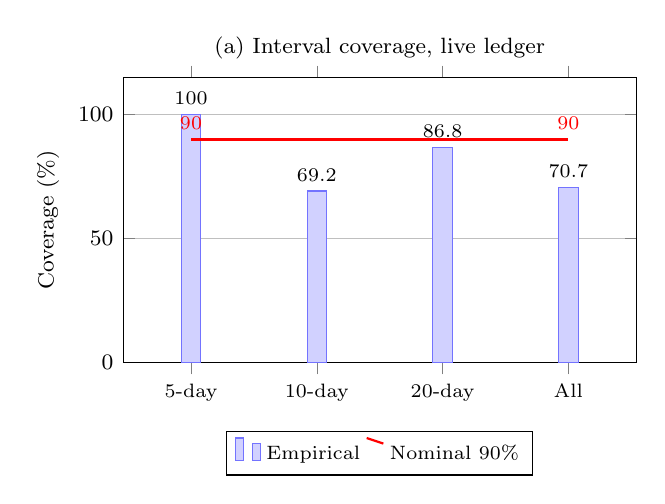
\begin{tikzpicture}
\begin{axis}[
  width=8.1cm, height=5.2cm, font=\footnotesize,
  ybar, bar width=7pt,
  symbolic x coords={5-day,10-day,20-day,All},
  xtick=data, x tick label style={font=\scriptsize},
  ymin=0, ymax=115, ylabel={Coverage (\%)},
  enlarge x limits=0.18, ymajorgrids,
  legend style={at={(0.5,-0.24)},anchor=north,legend columns=2,font=\scriptsize},
  nodes near coords, every node near coord/.append style={font=\scriptsize},
  title={(a) Interval coverage, live ledger}, title style={font=\footnotesize,yshift=-1mm}
]
\addplot[fill=blue!18,draw=blue!55] coordinates {(5-day,100.0)(10-day,69.2)(20-day,86.8)(All,70.7)};
\addplot[sharp plot,thick,red,mark=none,update limits=false] coordinates {(5-day,90)(All,90)};
\legend{Empirical, Nominal 90\%}
\end{axis}
\end{tikzpicture}%
\hspace{8mm}%
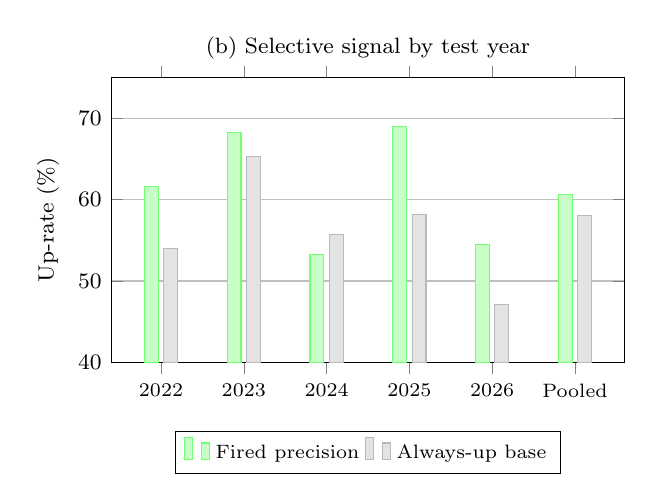
\begin{tikzpicture}
\begin{axis}[
  width=8.1cm, height=5.2cm, font=\footnotesize,
  ybar, bar width=5pt,
  symbolic x coords={2022,2023,2024,2025,2026,Pooled},
  xtick=data, x tick label style={font=\scriptsize},
  ymin=40, ymax=75, ylabel={Up-rate (\%)},
  enlarge x limits=0.12, ymajorgrids,
  legend style={at={(0.5,-0.24)},anchor=north,legend columns=2,font=\scriptsize},
  title={(b) Selective signal by test year}, title style={font=\footnotesize,yshift=-1mm}
]
\addplot[fill=green!22,draw=green!55] coordinates {(2022,61.6)(2023,68.3)(2024,53.3)(2025,69.0)(2026,54.5)(Pooled,60.6)};
\addplot[fill=gray!22,draw=gray!55] coordinates {(2022,54.0)(2023,65.3)(2024,55.7)(2025,58.2)(2026,47.1)(Pooled,58.0)};
\legend{Fired precision, Always-up base}
\end{axis}
\end{tikzpicture}
\end{document}
